\chapter{Approaches}

\section{Preprocessing}

Before starting to build a \acrshort{nlp} model it's mostly inevitable to preprocess the data you want your model to rely on. In many
\acrlong{ml} projects preprocessing is the most important part. A solid data basis can increase the performance of the model. Further
more it's very likely that preprocessed data is much more comfortable to deal with than raw data.

\subsection{Collecting Data}

As mentioned in \ref{chap:data-source} the source data is stored in two separate \acrshort{pst} files. To extract information out of this
proprietary file format a library called \emph{pypff}\footnote{Available at \url{https://github.com/libyal/libpff/wiki/Python-development}}
is used. The email messages are stored in different directories which either can have multiple sub-folders inside. Because of this structure
a recursive approach fits best to collect the data. Listing \ref{code:traverse} shows the detailed implementation including the calls to
parse (:13) and clean (:15) the message at the same iteration. The parser consists of three independent routines to get the message string
from HTML, RTF, and plain text emails. The cleansing procedure is explained in the next section.

\subsection{Data Cleansing}

As seen in section \ref{chap:typical-contents} there is a huge part of messages which shouldn't be used for further processing. This messages
should be cleared from the message pool. This discipline is called \emph{data cleansing} and can save a lot of time later on the project if
it's done carefully. But not all messages need to be removed completely from the data set. There exist a few cases where it's possible to only
remove certain pieces of a message like signatures or the forwarded parts which are added by default if you reply to an e-mail.

Listing \ref{code:regular-expressions} shows a sample of the used regular expressions to detect unwanted content within the messages. If a
junk pattern (:1-3) matches, the whole message is deleted. The forwarded parts of messages, which are often displayed as citations, are stripped
off with several patterns (:5-10). The regular expressions are made out of observations during the exploration of the data sources.

\begin{lstlisting}[language=Python, label={code:regular-expressions}, caption=Regular expressions for junk detection]
JUNK_1 = re.compile('^Fehler bei der Nachrichtenzustellung')
JUNK_2 = re.compile('^Submitted on(.)*Submitted values are:')
JUNK_3 = re.compile('^Form Returned: Telefonnotiz')

FORW_1 = re.compile(r"[-]{5}\s*(Message d'origine)\s*[-]{5}")
FORW_2 = re.compile(r'[-]{5}\s*Weitergeleitete Nachricht\s*[-]{5}')
FORW_3 = re.compile(r'Am \d{2}.\d{2}.(20)?\d{2} (um )?\d{2}:\d{2}')
FORW_4 = re.compile('Von:(.)*An:|From:(.)*To:')
FORW_5 = re.compile('Submitted on(.)*Submitted values are:')
FORW_6 = re.compile('GB Digitaler Kundensupport <(.)*> schrieb am')
\end{lstlisting}

Further showed the exploration that messages with a length of more than 3000 characters\footnote{The remaining length after stripping off signatures
and forwarded parts} are principally newsletters or spam. On the other hand messages with a remaining length of less than 75 characters aren't of
interest as well. Therefore only messages between these two boundaries are chosen for further processing steps.

The email messages are written mostly in German but you can find some other languages like French, Italian, and English in the raw data. The final
model should be able to predict named entities in German but not in foreign languages which would require a lot more training data and knowledge about
these languages. A data scientist at Swiss Mobiliar recently developed a library which combines four language recognition methods to predict the
language of a given text by simply calling all four functions and returning the language with the most votes. This library got the appropriate name
\emph{LangVoter} and is used to filter out any non-German messages.

After data cleansing the number of messages is sharply below the original amount. More than 55 percent of messages have been cleaned (see Figure
\ref{fig:plot-comparison-cleansing}). Figure \ref{fig:plot-comparison-cleansing-types} shows that the remaining data set consists of 10830 HTML
(-48\%), 949 plain text (-83\%), and 378 RTF messages (-60\%). As mentioned in section \ref{chap:data-source} many auto-generated messages are of
type RTF and plain text. Therefore it isn't surprising at all that most plain text and the bigger part of RTF messages don't contain valuable
information for the training of a \acrlong{ner}.

A reliable deep learning model should be trained with as many samples as possible to give reasonable predictions. With a total amount of 12157
messages and the right techniques to virtually increase the training set size, this might be enough for the beginning.

\begin{figure}[!ht]
    \begin{subfigure}{0.5\textwidth}
        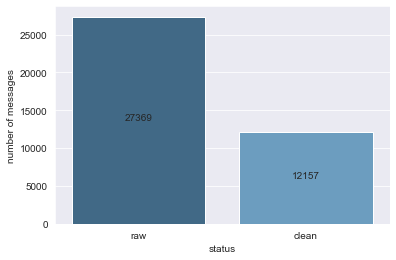
\includegraphics[scale=0.4]{plot-comparison-cleansing-total}
        \caption{Comparison in general}
        \label{fig:plot-comparison-cleansing}
    \end{subfigure}
    \begin{subfigure}{0.5\textwidth}
        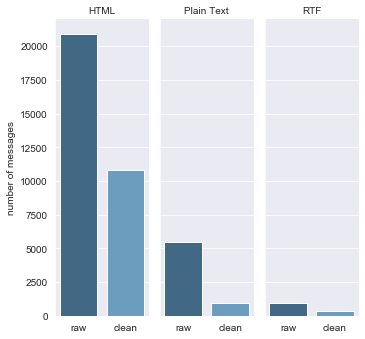
\includegraphics[scale=0.4]{plot-comparison-cleansing-type}
        \caption{Comparison grouped by type}
        \label{fig:plot-comparison-cleansing-types}
    \end{subfigure}
    \caption{Comparison before and after data cleansing}
\end{figure}


\subsection{Data Labelling}

In supervised learning a model needs to know the correct classification of the samples to compare them against its own predictions. The data set
is called pre-labelled. An inevitable part of a data scientist's work is to label data manually. Doccano\footnote{available at
\url{https://doccano.herokuapp.com}} is an open-source text annotation tool built for creating labelled data. It supports sequence to sequence
labelling which is useful for \acrlong{ner}.

\subsubsection{Doccano Parser}

One downside of Doccano are the limited options for exporting labelled data. You can download data only as JSON file with text labels. The exported
file has the same structure as listing \ref{code:doccano-export}. If the exported data should be used as validation set it needs to become more
handy to work with. Therefore I created a python library called \emph{mobi\_docparser}. The library allows users to parse Doccano's offset notation
into a list with two elements: The text after a simple whitespace tokenisation and the corresponding labels for each token, either in \acrshort{iob}
or binary notation. After parsing, the named-entity \emph{vodka martini} would be splitted into the tokens \emph{vodka} (B-DRINK) and \emph{martini}
(I-DRINK).

\begin{lstlisting}[label={code:doccano-export}, caption=Sample export from Doccano as JSON (text labels)]
{
  "id": 12162,
  "text": "Bond drinks his vodka martini shaken, not stirred.",
  "meta": {},
  "annotation_approver": null,
  "labels": [[0, 4, "per"], [16, 29, "drink"]]
}
\end{lstlisting}

\section{SpaCy Model}

SpaCy is meant to be the fast and easy-to-use \acrshort{nlp} library for the industry. Unlike more scientific libraries like NLTK\footnote{For more
information consider \url{https://www.nltk.org}}, spaCy focuses on getting work done rather than optimizing parameters to achieve even better results.
It's shipped with support for more than 53 languages including \acrlong{ner}, pretrained word vectors, and a non-destructive tokenization\footnote{
SpaCy's tokenization is fully reversible to reconstruct the original text} \cite{spacy}.

\subsection{Implementation}

Like the developers of spaCy mentioned on their homepage, it's very easy to integrate spaCy into your project. With just a few lines of code a pretrained
language model can process input texts.

\begin{lstlisting}[language=Python, label={code:spacy-integration}, caption=Sample of a runnable spaCy model]
import spacy

# load the German language model
nlp = spacy.load('de_core_news_md')

# process text
doc = nlp('Bond drinks his vodka martini shaken, not stirred.')

for token in doc:
    # print named-entities
    print(token.ent_type_)
\end{lstlisting}

There exist three German language models which can be used to process text. As seen in listing \ref{code:spacy-integration} (line 4) the medium-sized
news model is being used for this baseline approach. The model has a size of 214 MB and is able to recognise \emph{LOC}, \emph{MISC}, \emph{ORG}, and
\emph{PER} entities \cite{gh-spacy}. It's trained with data sources from the \emph{TIGER Corpus} and \emph{WikiNER}. The former has been trained with
approximately 50 000 sentences from the \emph{Frankfurter Rundschau} newspaper \cite{tiger}.

The \emph{WikiNER} corpus represents 7200 manually-labelled Wikipedia articles including the nine largest Wikipedias including English, German, Spanish,
and French. Unlike the \emph{TIGER Corpus}, the data quality of \emph{WikiNER} is only silver-standard. This means that the data is automatically created
by exploiting Wikipedia. Every link inside an article is getting replaced by the manually-labelled \acrshort{ne} category of the linked article \cite{Nothman}.

\subsection{Validation}

To validate spaCy's predictions the results need to be compared against the labelled \gls{mobi24} data. Because of the more sophisticated tokenisation
process of spaCy, the tokens aren't comparable with the output of the \emph{mobi\_docparser} library. Therefore spaCy's default tokenizer needs to be
overwritten with a simple whitespace tokenizer. As seen in listing \ref{code:tokenizer} the custom tokenizer simply uses the \verb|split()| function of
python's string module \cite{spacy-tok}.

\subsection{Performance}



this is what I got so far as results:

Values for NER only with PER:
    Accuracy 0.9604750950612733
    Precision 0.45423386721729264
    Recall 0.5127429916103949
    
Values for NER with LOC:
	Accuracy 0.9702884543615491
	Precision 0.05402757788198153
	Recall 0.03206319974275776

\subsection{Conclusion}

show advantages and disadvantages of spacy
why is it so low? what's the problem? the corpora isn't suitable for swiss addresses and many names

\section{Regex Model}
\label{chap:regex-model}
A written language consists of a word set and a rules set to describe how single words can be combined together to form larger constructs
like sentences or even texts. Every language follows a specific pattern which changes a lot over time. In information technology, there exist
regular expressions\footnote{Patterns for defining character sequences used for search, replace or validation operations} which are very useful
to locate such patterns inside text.

A basic implementation of a regular expression based algorithm for \acrlong{ner} may sound very costly if you have to define every language rule
as a regular expression. But it can be simplified by the use of reference data. These kinds of data are called dictionaries and let you lookup
certain words to classify them according to the dictionary they are part of. This seems to be a very solid basis for classifying text. But because
of word ambiguity it's very important to define how to proceed if a term occurs in multiple dictionaries and not to rely simply on dictionaries.

\subsection{Basic Implementation}



\subsubsection{Dictionary Lookup}

This model uses several dictionaries to classify the tokens.

\subsection{Enhancements}

\subsection{Performance}

\subsection{Conclusion}

what's good?

